\documentclass[12pt, a4paper]{article}

\usepackage[utf8]{inputenc}
\usepackage[spanish]{babel}
\usepackage{geometry}
\usepackage{titlesec}
\usepackage{enumitem}
\usepackage{array}% antes de xcolor[table]/colortbl (necesario para columnas p{...})
\usepackage[table]{xcolor}
\usepackage{graphicx}
\usepackage{float} % entorno figure con [H]
\usepackage{fancyhdr}
\usepackage{hyperref}% casi el último paquete

\geometry{margin=2.5cm}

\definecolor{azulprincipal}{RGB}{30, 90, 160}
\definecolor{verdeexito}{RGB}{76, 175, 80}
\definecolor{tabheadfill}{RGB}{232, 196, 160}
\definecolor{tabheadtext}{RGB}{120, 70, 30}
% Sin columnas p{...}: en algunas instalaciones babel español + colortbl rompe \@mkpream (\insert@pcolumn).
\newcommand{\celdarep}[2]{\parbox[t]{#1}{\raggedright #2}}

\titleformat{\section}{\Large\bfseries\color{azulprincipal}}{}{0em}{}[\titlerule]
\titleformat{\subsection}{\large\bfseries\color{azulprincipal}}{}{0em}{}
\titleformat{\subsubsection}{\normalsize\bfseries\color{azulprincipal}}{}{0em}{}

\pagestyle{fancy}
\fancyhf{}
\rhead{\textit{Space Invaders — Documentación final}}
\lhead{\textit{Grupo Cachopin}}
\cfoot{\thepage}

\hypersetup{colorlinks=true, linkcolor=azulprincipal, urlcolor=azulprincipal}

\begin{document}

% ---------- PORTADA ----------
\begin{titlepage}
    \centering
    \vspace*{1.5cm}

    {\LARGE \textbf{SPACE INVADERS}}\\[0.4em]
    {\large Programación Orientada a Objetos (Java)}\\[2em]

    {\large \textbf{Sprint: Demo Day + entrega en eGela}}\\[0.3em]
    {\large \textit{Documentación final}}\\[2.5em]

    {\textbf{Grupo: Cachopin}}\\[0.5em]
    {\large \today}

    \vfill

    {\normalsize Estructura según entrega final (Apartados a, b, c, f, g, h).}\\[0.5em]
    {\small Los informes de MVC/patrones y de uso de LLM se entregan como documentos aparte.}

    \vspace{1.5cm}

    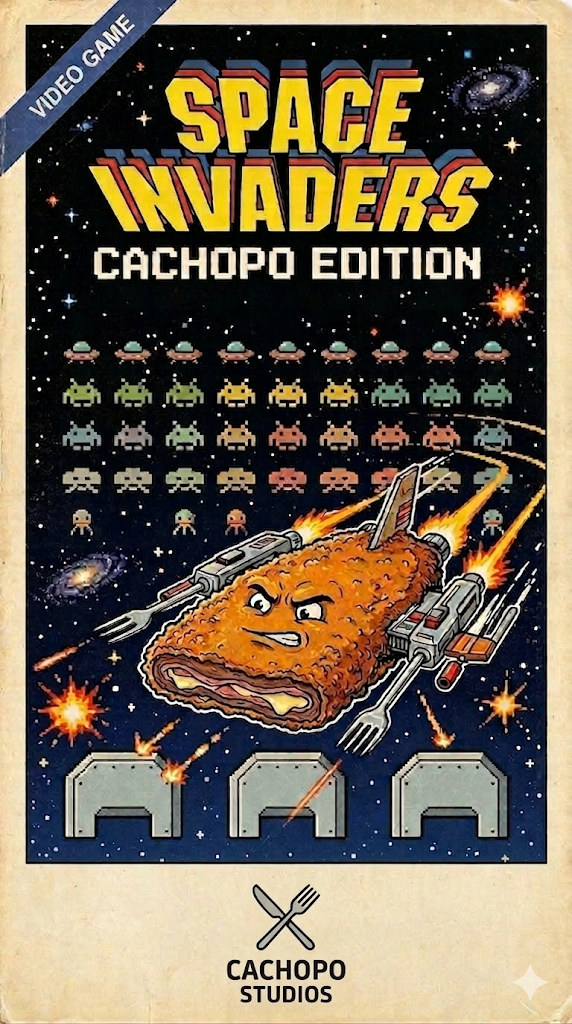
\includegraphics[width=3.2cm]{../PORTADA.png}

\end{titlepage}

\newpage
\tableofcontents
\newpage

% ============================================================
% a. Introducción → Presentación y objetivos
% ============================================================
\section{Introducción: presentación y objetivos}

\subsection{Presentación del proyecto}

Space Invaders es un proyecto académico en Java que reproduce el juego clásico: una nave en una cuadrícula debe eliminar enemigos que descienden sin ser alcanzada. El trabajo se ha organizado en tres sprints con entregas incrementales y revisión tras cada uno.

\subsection{Objetivos}

Aplicar POO en equipo, implementar patrones de diseño (MVC+Observer, Factory, Strategy, Composite), trabajar con metodología ágil y entregar un producto jugable y bien documentado.

% ============================================================
% Uso de LLM (resumen alineado con el informe LLM)
% ============================================================
\section{Herramientas LLM y asistentes de IA}

En el desarrollo moderno de software, los \textbf{modelos de lenguaje de gran escala (LLM)} son herramientas que pueden mejorar la productividad y la velocidad de desarrollo. Durante \textit{Space Invaders} se utilizaron varias herramientas de este tipo.

Es importante aclarar que la \textbf{responsabilidad final del código y del diseño recae en el equipo de desarrollo}: los LLM y los asistentes del IDE fueron \textbf{complementarios}, no sustitutos del criterio humano ni de la implementación supervisada.

\subsection{Herramientas utilizadas}

Visual Studio Code + GitHub Copilot, Cursor, Gemini y Claude para asistencia durante el desarrollo.

\subsection{Uso en el proyecto}

Las herramientas más usadas fueron los IDE con asistente de IA: autocompletado para código repetitivo, adaptación de clases, formato de documentos. La lógica compleja del juego y todas las sugerencias fueron supervisadas antes de integrar.

\subsection{Generación de imágenes}

Se utilizó Gemini para generar los fondos del juego con temática cachopo-nave en estilo pixel art.

\begin{figure}[H]
    \centering
    
\includegraphics[width=0.72\textwidth]{imgs/fondo2.png}
    \caption{Fondo del juego generado con Gemini: temática \textit{cachopo-nave} en estilo pixel art.}
    \label{fig:fondo2-gemini}
\end{figure}

% ============================================================
% b. Gestión → Reparto de tareas, reuniones y recursos
% ============================================================
\section{Gestión: reparto de tareas, reuniones y recursos}
\label{sec:gestion}

\subsection{Metodología}

Se ha seguido un esquema ágil: sprints de 2-3 semanas, demos y revisión con el cliente (profesorado) tras cada entrega. Uso de Git para versionado del código, reuniones de equipo y integración frecuente.

\subsection{Equipo}

El trabajo se ha distribuido entre cuatro miembros: \textbf{Unai Urrutia}, \textbf{Ekain Ortega}, \textbf{Eder Lorenzo} y \textbf{Asier López}. Cada uno ha contribuido en modelo, vista, controlador, integración y documentación según las necesidades de cada sprint.


% ============================================================
% f. Desarrollo → Para cada Sprint objetivos y decisiones
% ============================================================
\section{Desarrollo: objetivos y decisiones por sprint}

\subsection{Sprint 1}

\textbf{Objetivos principales:}
\begin{itemize}[leftmargin=2em]
    \item Tener un \textbf{juego jugable mínimo}: nave, enemigo(s), disparo y condiciones de fin de partida.
    \item Establecer la \textbf{arquitectura base} del código y la división en capas de forma coherente.
    \item Fijar convenciones de paquetes, nombres y flujo de trabajo en Git.
\end{itemize}

\textbf{Decisiones clave:}
\begin{itemize}[leftmargin=2em]
    \item Matriz de $10 \times 10$ píxeles como tamaño del tablero de juego.
    \item Uso de \texttt{Timer} para movimiento de enemigos y disparos.
    \item Naves y enemigos como entidades multipixel usando Composite.
\end{itemize}

\subsection{Sprint 2}

\textbf{Objetivos principales:}
\begin{itemize}[leftmargin=2em]
    \item \textbf{Ampliar} funcionalidad: distintas naves, enemigos y disparos según requisitos del backlog.
    \item Refactorizar donde haga falta para mantener el código \textbf{mantenible} sin romper lo ya entregado.
\end{itemize}

\textbf{Decisiones clave:}
\begin{itemize}[leftmargin=2em]
    \item Patrón \textbf{Factory} para creación centralizada de naves (Nave1, Nave2, Nave3, Nave4).
    \item Patrón \textbf{Strategy} para tipos de disparo (Pixel, Flecha, Rombo, Doble).
    \item Patrón \textbf{Composite} para geometría variable de naves y enemigos.
\end{itemize}

\subsection{Sprint 3}

\textbf{Objetivos principales:}
\begin{itemize}[leftmargin=2em]
    \item Cerrar \textbf{historias de usuario} pendientes, pulir la experiencia de juego y la estabilidad.
    \item Completar \textbf{documentación final}, preparar \textbf{Demo Day} y entrega en eGela.
    \item Opcional: extensiones acordadas para la nota máxima (HU adicional), si aplica.
\end{itemize}

\textbf{Decisiones clave:}
\begin{itemize}[leftmargin=2em]
    \item Sistema de puntuación visible en pantalla.
    \item Pantalla final (FinalFrame) con opción de reinicio desde menú.
    \item Fondos de imagen para todas las pantallas.
\end{itemize}

% ============================================================
% g. Reparto de tareas* → Para cada Sprint
% ============================================================
\section{Reparto de tareas por sprint}
\label{sec:reparto}

El equipo ha documentado el reparto de tareas en cada sprint. Ver archivos \texttt{REPARTO TAREAS SPRINT1.tex}, \texttt{REPARTO TAREAS SPRINT2.tex} y \texttt{REPARTO TAREAS SPRINT3.tex} en \texttt{DOCUMENTOS/} para detalle completo.

\subsection{Sprint 1}

\textbf{Sprint 1:} 50 horas reales de desarrollo. Tareas clave: patrón MVC+Observer, clases principales del modelo, lógica de colisiones, interfaz gráfica.

\subsection{Sprint 2}

\textbf{Sprint 2:} 50 horas reales de desarrollo. Tareas clave: Factory, Strategy, Composite; 3 naves iniciales; 3 tipos de disparos; diagramas UML.

\subsection{Sprint 3}

\textbf{Sprint 3:} Desarrollo de funcionalidades adicionales (Nave4, DisparoDoble, sistema de puntuación, fondos, pantalla final mejorada) y documentación final.

% ============================================================
% h. Conclusiones → reflexión y cambios futuros
% ============================================================
\section{Conclusiones: reflexión y cambios futuros}

\subsection{Reflexión}

El proyecto ha permitido al equipo experimentar con programación orientada a objetos en un entorno colaborativo, aplicando patrones de diseño reales y metodología ágil. Los mayores desafíos fueron la integración entre patrones (Composite + Strategy), la coordinación de cambios simultáneos en Git y mantener la calidad del código conforme crecía en complejidad.

\subsection{Cambios y mejoras futuras}

Líneas de mejora futuras:

\begin{itemize}[leftmargin=2em]
    \item Pruebas unitarias (JUnit) para la lógica del modelo.
    \item Niveles de dificultad progresiva.
    \item Sonido y animaciones.
    \item Optimización de rendimiento si la complejidad del juego aumenta significativamente.
\end{itemize}

\vspace{2em}

\begin{center}
    \textcolor{verdeexito}{\textbf{Fin del documento (entrega documentación final + Demo Day).}}
\end{center}

\end{document}
